\section{Evolução dos materiais}
\subsection*{Idade da Pedra}
Materiais mais comuns: Polímeros (madeiram peles e fibras);Cerâmicos (Pedra)
\subsection*{Idade da Argila}
Materiais mais comuns: 
\subsection*{Idade do Cobre}
Materiais mais comuns: 
\subsection*{Idade do Bronze}
Materiais mais comuns: 
\subsection*{Idade do Ferro}
Materiais mais comuns: 
\section{Sociedade e Materiais}
Aumento significativo de tipos de materiais com o desenvolvimento industrial $\rhd$ Melhoria nos métodos de extração e produção \& Alterações nos materiais para formação de novos materiais (materiais avançados, compósitos)
\section{Classificação dos Materiais}
\subsection*{Metais}
Combinação de elementos metálicos, sendo possível a presença de não-metálicos (ex: aço-carbono).Algumas propriedades relacionadas à presença de elétrons livres (ex: bons condutores de calor e eletricidade).Resistentes e deformáveis: extenso uso em aplicações estruturais.
Suscetível a corrosão.

Possui boa condutividade térmica e elétrica.
\subsection*{Cerâmicos}
ligações de metais e não-metais. Isolantes térmicos e elétricos. Podem ser resistentes a altas temperaturas e a ambientes agressivos. Ex: óxidos, nitretos, carbetos.
Resistentes a corrosão.

Possui boa condutividade térmica e variada condutividade elétrica.

\subsection*{Polímeros}


polímeros:compostos orgânicos. Baixa densidade; altamente deformáveis. (C, H e não-metálicos)
Degrada com solventes, altas temperaturas.

Possui baixa condutividade térmica e elétrica.

\subsection*{Compósitos}

Compósitos: dois ou mais tipos de materiais unidos de forma a produzir um material com características específicas. Projetados para apresentar uma combinação das melhores características de cada um dos componentes.

\subsection*{Materiais avançados}

Uso em aplicações de ponta(alta tecnologia). Não necessariamente são novos materiais. Podem ser tradicionais, com otimização das propriedades.

\begin{itemize}
		
	\setlength{\parskip}{0pt}
	\setlength{\itemsep}{0pt plus 1pt}
	
\item Alto desempenho
\item Baixo peso e alta resistência
\item Resistência a diversas condições de serviço
\item Ambientalmente corretos
\item Facilmente recicláveis
\end{itemize}
Ex: polímero reforçado com fibra de vidro usado como armadura para estruturas em concreto armado


\section{Classificação dos Materiais}

\subsection*{Qaunto a Estrutura}

\begin{itemize}
		
	\setlength{\parskip}{0pt}
	\setlength{\itemsep}{0pt plus 1pt}
	
	\item Ligações atômicas
	
	\begin{itemize}
			
		\setlength{\parskip}{0pt}
		\setlength{\itemsep}{0pt plus 1pt}
		
		\item Metálica
		\item covalente
		\item iônica
	\end{itemize}

	\item Tipo de Estrutura
	\begin{itemize}
			
		\setlength{\parskip}{0pt}
		\setlength{\itemsep}{0pt plus 1pt}
		
		\item Amorfa
		\item Cristalina
		\item Molecular
	\end{itemize}
\end{itemize}


\subsection*{Propriedades Mecânicas}
\begin{itemize}
		
	\setlength{\parskip}{0pt}
	\setlength{\itemsep}{0pt plus 1pt}
	
	\item dutilidade
	\item elasticidades
	\item dureza
	\item tenacidade
\end{itemize}

\subsection*{Propriedades Químicas e Físicas}
\begin{itemize}
		
	\setlength{\parskip}{0pt}
	\setlength{\itemsep}{0pt plus 1pt}
	
\item	ponto de fusão
\item	calor específico
\item	condutividade (térmica e elétrica)
\item 	Propriedades magnéticas
\item 	Propriedades ópticas
\item 	Iteração com o ambiente: oxidação 
\end{itemize}

\subsection*{Modificação das Propriedades}
\begin{itemize}
		
	\setlength{\parskip}{0pt}
	\setlength{\itemsep}{0pt plus 1pt}
	
	\item Tratamentos térmicos
	\item tratamento de superfície
	\item Tratamentos mecânicos
\end{itemize}


\section{COMPOSIÇÃO QUÍMICA x PROPRIEDADES FÍSICAS}
Exemplo 1: alteração de cor de um mesmo mineral

CORÍNDON:mineral à base de óxido de alumínio (Al2O3)
Chama-se safira qualquer variedade de corindon, de qualidade gemológica, que não seja vermelha (rubi)

Exemplo 2: Alteração da compatibilidade química com o meio ambiente.
Aço patinável (CORTEN): aço com adição de cobre que forma uma pátina, reduzindo o processo corrosivo. Muito usado na construção civil.



\section{ESTRUTURA CRISTALINA x PROPRIEDADES FÍSICAS}
CaCO3

Mármore (calcita -romboédrico)

Conchas (aragonita -ortorrômbico)

\section{TIPO DE LIGAÇÃO QUÍMICA x PROPRIEDADES FÍSICAS}

O tipo de ligação iônica está intimamente ligada com as características físico-química dos materiais.

Temos que:
\subsection*{Ligações Metálicas}
Favorecem a condutividade térmica e elétrica

\subsection*{Ligações Covalentes}
Aparecem em matérias com características isolantes. 


\section{Materiais de Construção}

\subsection*{Escolha do Material}

Etapas básicas

\begin{itemize}
	
\setlength{\parskip}{0pt}
\setlength{\itemsep}{0pt plus 1pt}

\item relacionar experiências prévias para o serviço em questão
\item relacionar e colocar em ordem de prioridade todos os parâmetros que podem influenciar na escolha
\item estabelecer as características que se deseja para o material ideal ao serviço
\item realizar testes, comparando os materiais que possam ser usados otimizando o custo total.

\end{itemize}

Definição da categoria do material: metal, cerâmico, polímero ou compósito

\subsection*{Como selecionar um material?}

Condições operacionais
\begin{itemize}
	
	\setlength{\parskip}{0pt}
	\setlength{\itemsep}{0pt plus 1pt}
	
\item Custo/benefício (indústria de massa ou de grande exigência tecnológica?)
\item Propriedades requeridas
\item Degradação no meio
\item Solicitação mecânica
\item Resistência/peso
\end{itemize}

\subsection*{Quais fatores influenciam na escolha dos materiais para determinado serviço ou aplicação industrial?}

\begin{itemize}
	\setlength{\parskip}{0pt}
	\setlength{\itemsep}{0pt plus 1pt}
	
	\item Propriedades físicas e químicas 
	\item Características operacionais
	\item Fabricação, disponibilidade e custo
	
\end{itemize}


\section{Propriedades físicas e químicas}

\subsection*{Propriedades mecânicas}
Limites de escoamento e de resistência, dutilidade, resistência à fadiga e fluência, temperatura de transição dútil-frágil, módulo de elasticidade.

\subsection{Outras propriedades físicas}
densidade, calor específico,expansão térmica,condutividade,propriedades magnéticas e elétricas.


\subsection*{Propriedades químicas}
oxidação, flamabilidade,toxicidade.

\section{Características operacionais}

\subsection*{temperatura}

\subsection*{natureza dos fluidos em contato com material}

(composição química, concentração, pH, caráter oxidante ou redutor, presença de contaminantes, pressão, velocidade do fluido, flamabilidade, toxidez). Necessário avaliar alterações em cada um destes fatores ao longo do tempo de serviço.

\subsection*{presença de resíduos oriundos de processos corrosivos}
ex: alguns materiais como o chumbo são resistentes à corrosão porém geram resíduos tóxidos, limitando seu uso.

\section{Fabricação,disponibilidade e custo}


\subsection*{Fatores críticos na seleção:} facilidade de fabricação e forma de apresentação. Ex:espessura de chapas e formato(tubos ou tarugos)
Custo/benefício: custo direto do material, tempo de vida útil e custos indiretos (paradas para reparos ou reposição dos equipamentos).
Tempo de vida útil compatível com tempo previsto de operação.
Relação direta com segurança (acidentes e falhas)
Furos em tubulações.
Aço inox 304 no lugar de aço-C.
Aço-carbono disponível em inúmeras formas de fabricação.


\section{Estrutura Cristalina}

\subsection*{Material Amorfo X Cristalino}
O material CRISTALINO possui arranjo mais uniforme e as moléculas está direcionadas de forma a apresentarem um densidade molecular maior. 

O material AMORFO possui suas moléculas dispostas de forma mais aleatória e a densidade molecular dessa região é menor.


\subsection*{CRISTALINIDADE} Arranjo interno ordenado das partículas segundo um modelo tridimensional, característico do estado sólido. Em muitos corpos a cristalinidade é evidenciada por faces e simetria externa, indicando um arranjo ordenado dos átomos. Exames em raios X(1912) estudo de substâncias inorgânicas.

\subsection*{CRISTALOGRAFIA} Estudo dos corpos sólidos que possuem estrutura cristalina e das leis que governam seu crescimento, forma externa e interna. É instrumento fundamental na química, física, metalurgia e no estudos das cerâmicas, refratários, semicondutores, gemas sintéticas, etc.


\subsection*{CÉLULAS UNITÁRIAS} para a maioria dos cristais, as células unitárias podem ser representadas por geometrias específicas. Mais do que uma célula unitária pode ser escolhida para representar o cristal. Geralmente, escolhe-se a que apresenta o maior grau de simetria geométrica.



\subsection*{SISTEMAS CRISTALINOS} Qualquer empacotamento atômico deverá se encaixar em um dos sete principais tipos de cristais, que estão intimamente associados com o modo pelo qual o espaço pode ser dividido em volumes iguais, pela interseção de superfícies planas.
Existem diferentes estruturas cristalinas possíveis. É conveniente dividi-las em grupos de acordo com as configurações das células unitárias e/ou os arranjos atômicos. Para criar todos os tipos de redes são necessários sete tipos distintos de células cristalinas.


\section{Células unitárias e Sistemas cristalinos}

Parâmetros de rede cristalina:
\begin{itemize}
	\setlength{\parskip}{0pt}
	\setlength{\itemsep}{0pt plus 1pt}
	
	\item a,b,c - comprimentos dos lados do paralelepípedo
	\item $ \alpha$, $\beta$, $\gamma $ - ângulos entre os eixos
\end{itemize}




Com base nestes parâmetros de rede, tem-se que existem 7 diferentes combinações possíveis entre a,b,c e $\alpha, \beta, \gamma $ cada um representando um sistema cristalino.


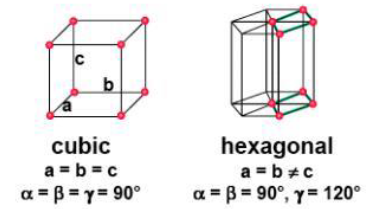
\includegraphics[scale=0.5,trim={0 0 0 0}]{figures/crist1}

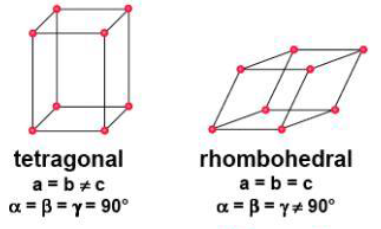
\includegraphics[scale=0.5,trim={0 0 0 0}]{figures/crist2}

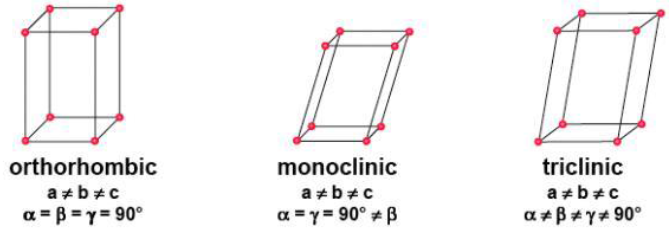
\includegraphics[scale=0.3,trim={0 0 0 0}]{figures/crist3}


O maior grau de simetria aparece no sistema cúbico e o menor grau é visto no sistema triclínico.

\subsection*{Variações na célula unitária básica}

As possíveis redes podem ser descritas por 14 células unitárias (A.J. Bravais).
Em algumas células unitárias existem alguns tipos básicos: simples, de corpo centrado e de faces centradas.
 
 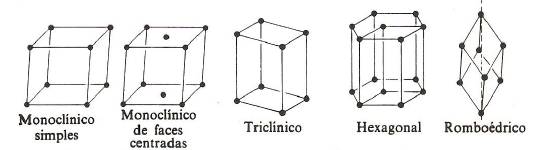
\includegraphics[scale=0.4,trim={0 0 0 0}]{figures/var1}
 
 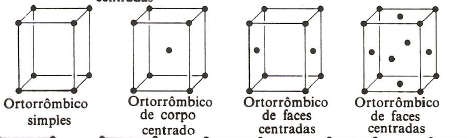
\includegraphics[scale=0.45,trim={0 0 0 0}]{figures/var2}
 
 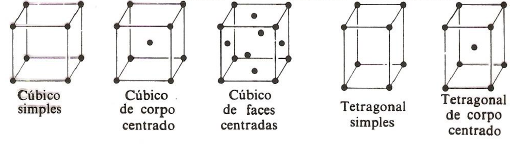
\includegraphics[scale=0.5,trim={0 0 0 0}]{figures/var3}



\subsection*{Características}

Numero de Coordenação: número de partículas que envolvem uma partícula central.

Fator de empacotamento: volume de átomos numa célula unitária / volume da célula unitária.

\subsection*{Valores para alguns sistemas cristalinos}

\begin{itemize}
	\setlength{\parskip}{0pt}
	\setlength{\itemsep}{0pt plus 1pt}
	
	\item NC: Número de Coordenação
	\item FE: Fator de empacotamento
\end{itemize}


Cubo simples - CS

%\begin{itemize}[noitemsep]
%	\item NC: 6;
%	\item FE: $\frac{4}{3} \cdot \frac{\pi \cdot r^{3}}{a^{3}} = 0,52$;
%	\item Rel: a = 2R;	
%\end{itemize}



\begin{itemize}
	\item NC: 6;
	\item FE: $\frac{4}{3} \cdot \frac{\pi \cdot r^{3}}{a^{3}} = 0,52$;
	\item Rel: $a = 2R$;	
\end{itemize}


Cúbico de Corpo Centrado - CCC

\begin{itemize}
	\item NC: 8
	\item FE: $2 \cdot \frac{4}{3} \cdot \frac{\pi \cdot r^{3}}{a^{3}} = 0,68$
	\item Rel: $a = \frac{4R}{\sqrt{3}}$
\end{itemize}


Cúbico de Faces Centradas - CFC

\begin{itemize}
	\setlength{\parskip}{0pt}
	\setlength{\itemsep}{0pt plus 1pt}
	
	\item NC: 12
	\item FE: $4 \cdot \frac{4}{3} \cdot \frac{\pi \cdot r^{3}}{a^{3}}$ 0,74
	\item Rel: a = $\frac{4 \cdot R}{\sqrt{2}}$
\end{itemize}

Hexagonal

\begin{itemize}
	
	\setlength{\parskip}{0pt}
	\setlength{\itemsep}{0pt plus 1pt}
	
	\item NC: 12
	\item FE: 0,73 (=CFC)
	\item Rel: a = 2R
\end{itemize}


 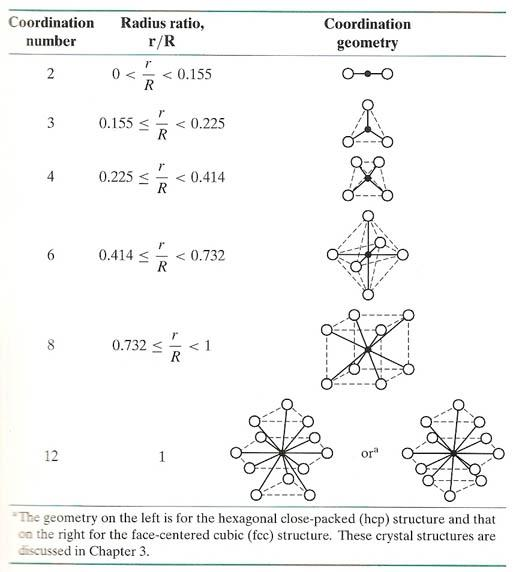
\includegraphics[scale=0.3,trim={0 0 0 0}]{figures/RELraio}
 
 
 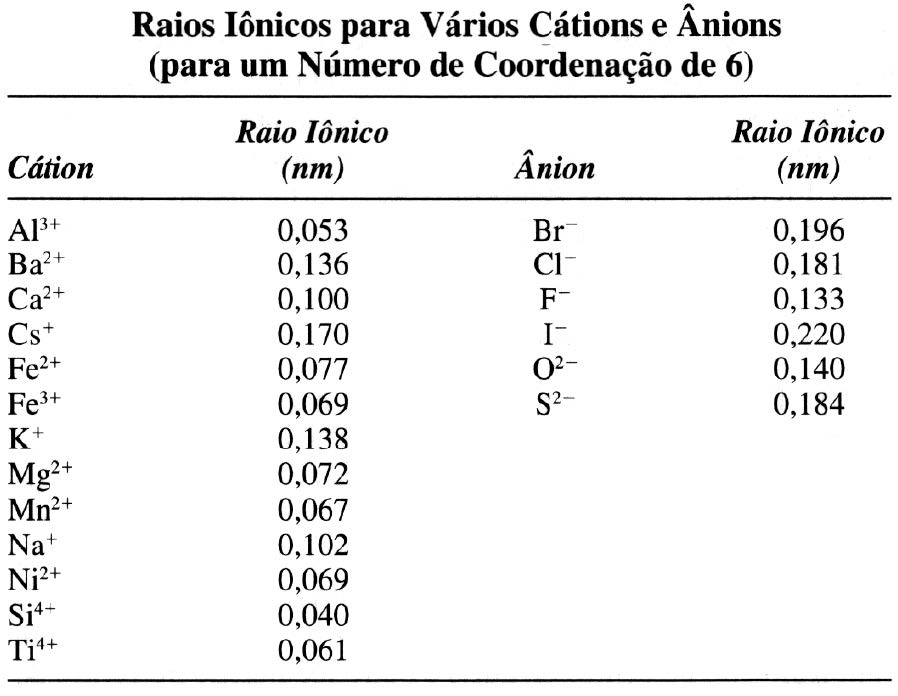
\includegraphics[scale=0.2,trim={0 0 0 0}]{figures/raio}
 

 \section{Estrutura dos materiais Cerâmicos}
 
O posicionamento das partículas nos materiais cerâmicos depende da relação entre os raios(cátion/ânion) e das cargas envolvidas. Nos vazios (sítios ou interstícios) da rede cristalina se posicionam partículas diferentes das que existem na rede cristalina principal. Em redes compactas há espaços intersticiais, onde as partículas ficam equidistantes do centro do espaço vazio.
 

\textbf{Posições octaédricas na rede cfc:}

 \begin{itemize}
 	
 	\setlength{\parskip}{0pt}
 	\setlength{\itemsep}{0pt plus 1pt}
 	
 	\item NC: 6
 	\item Local:arestas (3 sítios) + centro da célula unitária
 	\item Total: 4 partículas (1 por partículas da célula unitária)
 \end{itemize}

 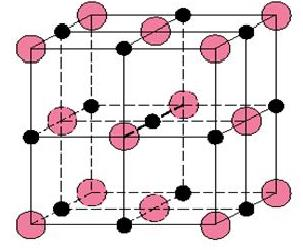
\includegraphics[scale=0.5,trim={0 0 0 0}]{figures/occfc}
 
 
\textbf{ Posições tetraédricas na rede cfc:}

  \begin{itemize}
 	
 	\setlength{\parskip}{0pt}
 	\setlength{\itemsep}{0pt plus 1pt}
 	
 	\item NC: 4
 	\item Local:posições do tipo ($\frac{1}{4}$, $\frac{1}{4}$, $\frac{1}{4}$)
 	\item Total: 8 partículas (2 por partículas	da célula unitária)
 \end{itemize}

 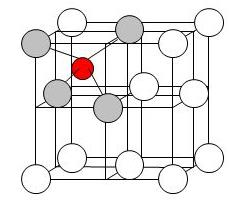
\includegraphics[scale=0.5,trim={0 0 0 0}]{figures/tetcfc}
 
\section{Estrutura dos Materiais Cerâmicos}
FEI=fator de empacotamento iônico
As estruturas são bastante complexas, podendo-se representar alguns tipos mais comuns:


\begin{itemize}
	\item Cerâmicostipo MaM’bXc
	\item $MX$
	\item $MX_{2}$
	\item $M_{2}X_{3}$
	\item $MM'X_{3}$
	\item $M'M_{2}''X_{4}$
\end{itemize}

M –elemento metálico

X–elemento não-metálico



Estrutura tipo MX -NaCl

Ex 1: NaCl (cfc)
NC = 6
A estrutura pode ser vista como duas estruturas CFC, uma de íons sódio e uma de íons cloro.
2 íons associados(1 Na+e 1 Cl-)
4 íons de cada (CFC –4 átomos por célula unitária)
São 8 íons por célula unitária.
Outros compostos com esta estrutura: CaO, NiO, FeO, MgO.

 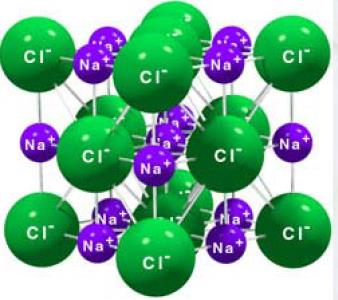
\includegraphics[scale=0.5,trim={0 0 0 0}]{figures/NaCl}


Estrutura tipo MX -CsCl
Ex2: CsCl(ccc)

Estrutura cúbica (NC = 8)

 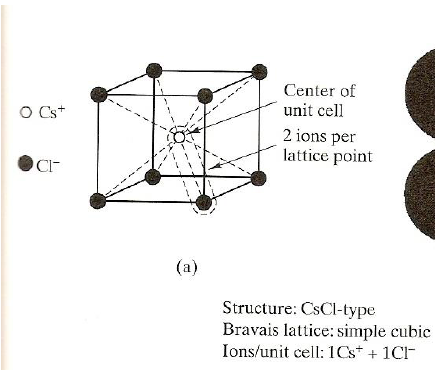
\includegraphics[scale=0.2,trim={0 0 0 0}]{figures/CsCl}
 
 

Estrutura tipo MX -ZnS
Ex3: ZnS(cfc)
cfc:8 íons por célula unitária (4 Zn2+e 4 S2-)
4 S2-em posição cfce Zn2+em 4 sítios tetraédricos
(1/2 dos sítios tetraédricos ocupados)

 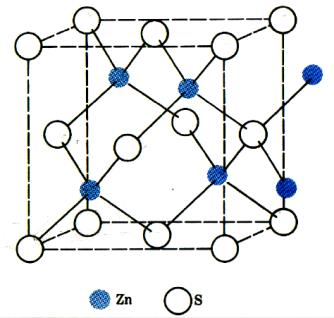
\includegraphics[scale=0.3,trim={0 0 0 0}]{figures/ZnS}


 Estrutura tipo MX2 –CaF2
 Ex: CaF2(cfc) -FLUORITA
 
3 íons associados ($1Ca^{+2} e 2F^{-}$)
4 íons Ca+2 (estrutura cfc) e 8 íons F-(12 íons por célula unitária)
Volume não preenchido próximo ao centro da célula unitária.

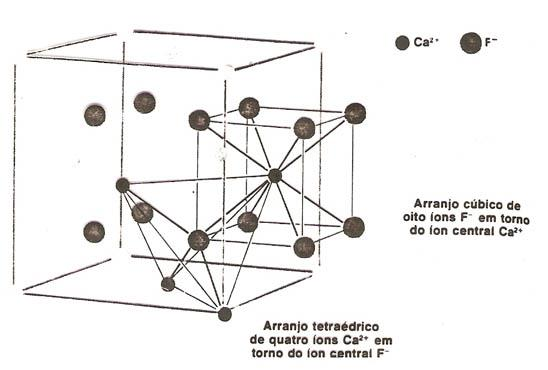
\includegraphics[scale=0.3,trim={0 0 0 0}]{figures/CaF2}

Estrutura tipo M2X3

Ex: Al2O3–alumina ou corundum
30 íons por célula unitária (12Al+3e18O2-)
2/3 dos interstícios ocupados por íons alumínio.
Outros compostos com esta estrutura:-Fe2O3,Cr2O3.
  
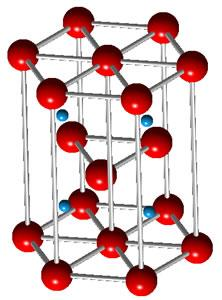
\includegraphics[scale=0.5,trim={0 0 0 0}]{figures/Al2O3}

Estrutura tipo MM'X3

 MeM'– elementos metálicos
 X –elemento não-metálico
 Ex: CaTiO3(combinação de estruturas cs, cc, cfc)–importante família de materiais cerâmicos usados na indústria eletrônica (propriedades piezoelétricas).
 Ca+2nos vértices, Ti+4como corpo centrado e O2-na faces.
 Este tipo de rede é um exemplo da estrutura CS formada pelos íons cálcio.
 Existem 5 íons por célula unitária (1Ca+2,1Ti4+e3O2)
 Outro composto com esta estrutura: BaTiO3.
 
  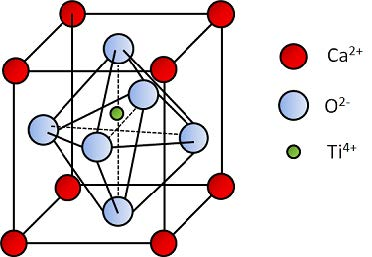
\includegraphics[scale=0.5,trim={0 0 0 0}]{figures/CaTiO}
  
  
Estrutura tipo MM2'X4

M(valência+2)eM'(valência+3)–elementos metálicos
X –elemento não-metálico
Ex: MgAl2O4(cfc)-importante família de materiais cerâmicos magnéticos (espinélios).
56 íons por célula unitária (8Mg+2,16Al3+e32O2-),
Outros compostos com esta estrutura: NiAl2O4,MgAl2O4,ZnFe2O4.

 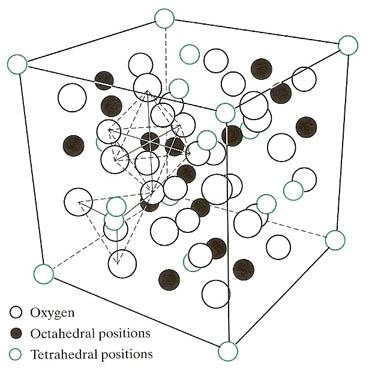
\includegraphics[scale=0.3,trim={0 0 0 0}]{figures/MgAlO}

\section{Estruturasdos Silicatos}
Formam a classe máxima entre os minerais.

\begin{itemize}
	\item A estrutura é complexa, não podendo ser definida como um tipo simples de estrutura, variando em função da temperatura e pressão.
	\item A característica geral dos silicatos é a mesma (tetraedros unidos) diferenciando em relação ao compartilhamento dos oxigênios.
\end{itemize}

Várias estruturas de silicatos surgem das diferentes maneiras segundo as quais unidades de (SiO4)-4 se unem formando arranjos unidimensionais, bidimensionais e tridimensionais.

Para Desenhar e anotar


Para os vários minerais à base de silicatos, 1, 2 ou 3 átomos de oxigênio nos vértices dos tetraedros são compartilhados por outros tetraedros para formar estruturas complexas.

Podem conter vários elementos em combinação com o silício e o oxigênio (ex: Na, K, Ca, Mg, Al e Fe).

 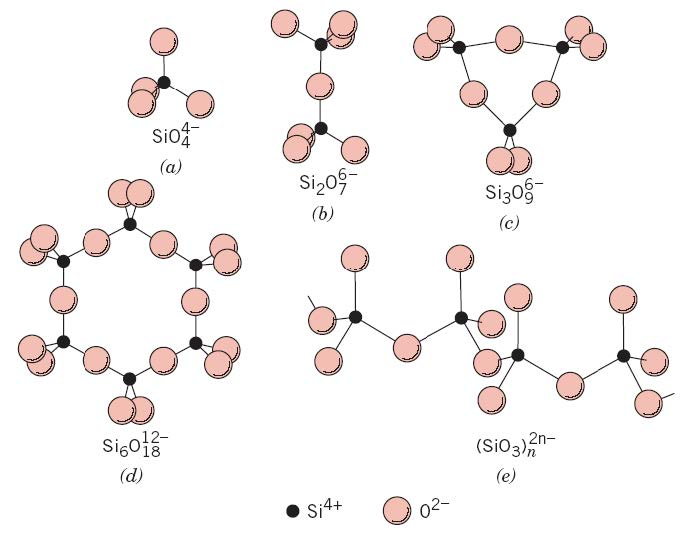
\includegraphics[scale=0.3,trim={0 0 0 0}]{figures/estsil}
  
 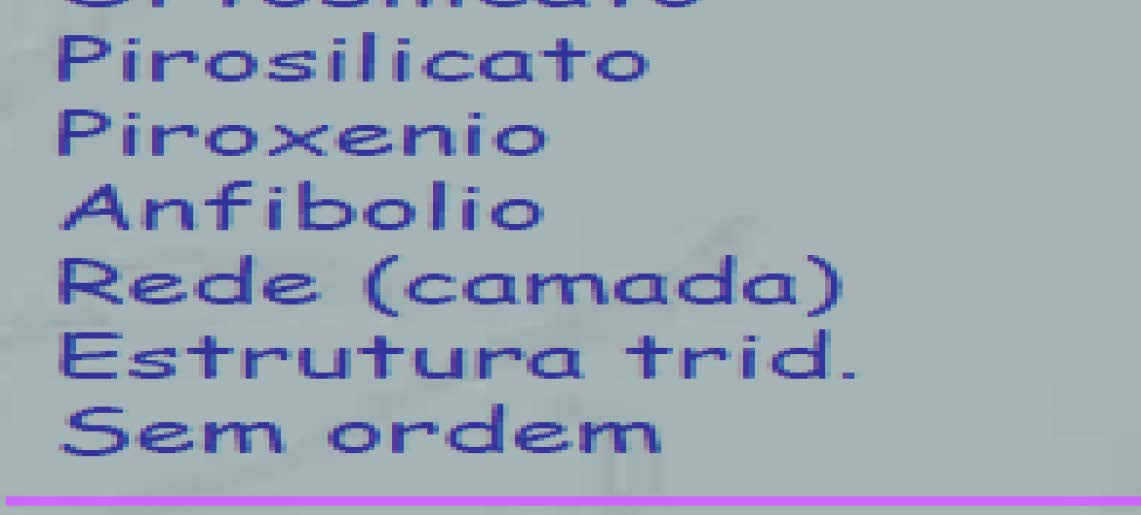
\includegraphics[scale=0.25,trim={0 0 0 0}]{figures/sil1}

\begin{itemize}
	\item tetraedros simples - ex: Mg2SiO4
	\item tetraedros duplos - ex: Zn4(Si2O7)(OH)2.H2O)
	\item anéis (unidade estrutural (SiO3)–2 )
	\item camadas - ex: talco: Mg3(Si2O5)2(H2O))
	\item redes (feldspatos, zeólitas, quartzo: SiO2) )
\end{itemize}

\textbf{Ex 1:SiO2(cfc) -CRISTOBALITA}
6 íons associados (2 Si+4e 4 O-2): Si2O4
24 íons por célula unitária(8 Si+4e 16 O-2)
Apesar da grande célula unitária necessária para descrever a estrutura, é uma das formas mais simples do SiO2.


\textbf{Ex2: Grupo dos feldspatos}

X Al(1-2)Si(2-3) O8


onde: Quando X tem carga +1, há 1Al e 3Si X = Na+, K+ou Ca2+ Quando X tem carga +2, há 2Al e 2Si. Quanto maior a quantidade de Ca, maior a quantidade de Al no feldspato. Os Si e os Al ocupam os centros de tetraedros interconectados. Os cátions X se situam nos vazios da estrutura.



\textbf{Ex3: Alumino-silicatos}
Alumínio pode entrar em Coordenação tetraédrica(em substituição ao Si) ou em Coordenação octaédrica, unindo tetraedros.
Mg2+, Fe2+, Fe3+, Mn2+, Al3+e o Ti4+tendem a ocorrer nas estruturas dos silicatos em coordenação octaédrica (em relação ao O2-).
Ca2+ (0,99 Å) e Na+(0,97 Å) (cátions maiores e de carga mais fraca) entram em coordenação cúbica (NC = 8).
Se um cátion trivalente substitui um tetravalente, ex: Fe3+na posição do Ti4+, outra substituição tem de ser feita no cristal de forma a perder uma carga positiva ou ganhar uma negativa eletroneutralidade.


\textbf{Ex4: Sílica vítrea}
SiO2 sem arranjo cristalino regular



\section{Formação de mamteriais cristalinos}
Materiais alotrópicos ou polimórficos apresentam mais de uma estrutura cristalina.

\textbf{Alotropia}: substâncias puras.

\textbf{Polimorfismo}: Substancias compostas

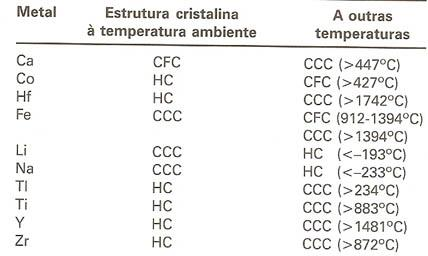
\includegraphics[scale=0.4,trim={0 0 0 0}]{figures/estruturaTemp}

O processo de formação de cristais pode ser através de processo natural, em laboratório ou na indústria.

O crescimento se dá sob forças acidentais, presença de íons estranhos, variação da temperatura.

Podem ainda ser feitor a partir:

\begin{itemize}
	\item Solução;
	\item Vapor;
	\item Massa em fusão.
\end{itemize}


Cada ponto de cristalização é chamado de núcleo de cristalização e a formação destes núcleos pode ser:

\begin{itemize}
	\item Homogênea: núcleos formados pelos átomos de próprio metal 
	\item Heterogênea: núcleos formados sobre um substrato ou outro material presente. Requer menor energia para formação de núcleo estável do que na própria substância.
\end{itemize}

A depender do número de núcleos presentes no material, este pode ser classificado como monocristalino e policristalino. As propriedades mecânicas podem variar de acordo com o número de núcleos cristalinos.

É observado experimentalmente que os materiais policristalinos apresentam defeitos, i.e. rachaduras e falhas, nas regiões entre os núcleos de cistalização.


\section{Soluções Sólidas}

Poucos metais são utilizados na sua forma pura. Sendo assim, grande parte dos materiais são chamados de ligas metálicas por haver combinação de dois ou mais metais.

Se o limite de solubilidade é ultrapassado, uma nova fase é formada e observada nesses materiais.

Exemplos de ligas metálicas:

\begin{itemize}
	\item Ligas de cobre: latão / bronze / cupro-níquel atãobronze
	\item Ligas de níquel: monel/ inconel/ incoloy
	\item Ligas ferrosas: Aço-C / Aços inoxidáveis
\end{itemize}

\section{Elementos de Liga}

Os elementos de liga são impurezas adicionadas intencionalmente e podem promover a melhora de algumas propriedades desses materiais e torná-lo útil para outras aplicações tecnológicas. Algumas características são:

\begin{itemize}
	\item dopagem em semicondutores;
	\item maior resistência mecânica;
	\item maior resistência a corrosão;
	\item maior condutividade elétrica;
	\item melhor soldabilidade.
\end{itemize}


\section{Soluções Sólidas}

Tipos de soluções sólidas:

\begin{itemize}
	\item substitucional: o átomo do elemento acrescido a liga substitui a posição de um dos átomos presentes na célula cristalina;
	\item intersticial: o átomo do elemento acrescido a liga invade o interstício dos átomos que formam a célula cristalina .
\end{itemize}


As soluções sólidas SUBSTITUCIONAIS podem ainda ocorrer de forma 

\begin{itemize}
	\item Ordenada;
	\item Ao acaso.
\end{itemize}

\section{Regras de Hume-Rothery}

\begin{itemize}
	\item Variação \% causada pela diferença entre raios < 15\% (evitar distorções na rede): raio soluto = raio solvente/
	\item Mesma estrutura cristalina;
	\item Eletronegatividades semelhantes
	\item Mesma valência.
\end{itemize}



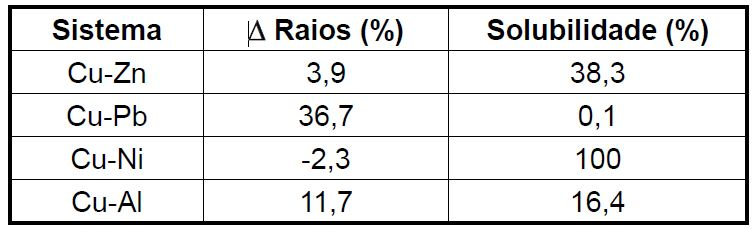
\includegraphics[scale=0.4,trim={0 0 0 0}]{figures/hume}


{\LARGE VER COMO É ESSA REGRA EM UM LIVRO DAS REF}

{\LARGE NECESSÁRIO TERMINAR ESSE TÓPICO COM FORMULAS}


\section{Imperfeições Cristalinas}

É uma imperfeição no arranjo periódico regular dos átomos em um cristal. Podem estar relacionada à posiçãodos átomos ou ao tipo de átomo presente na rede.

\textit{O tipo e o número de defeitos dependem do meio ambiente, do material e das circunstâncias sob as quais o cristal é processado.}

\begin{itemize}
	\item Representam pequena fração da rede mas podem significar muito nas propriedades dos materiais.
	\item Podem permitir a introdução de elementos de liga formando novos materiais.
\end{itemize}

Defeitos pontuais:

\begin{itemize}
	\item Lacunas ou vazios simples ou não.
	\item Originadas por perturbações locais durante a solidificação ou vibrações térmicas a altas temperaturas.
\end{itemize}

Defeitos em sólidos iônicos:

\begin{itemize}
	\item \textbf{Defeito de Schottky}: vazio de par de íons (exclusivo de materiais iônicos) AX $\rightarrow$par consistindo de lacuna de cátion e lacuna de ânion $\rightarrow$ neutralidade.
	\item \textbf{Defeito de Frenkel:} deslocamento de um íon para um interstício (muita energia adicional) $\rightarrow$lacuna de cátion + cátion intersticial $\rightarrow$Não existe alteração de cargaImperfeições
\end{itemize}


Contorno de grãos:

\begin{itemize}
	\item Formada entre cristais (contornos de grãos) ou nas superfícies externas.
	\item No contorno dos grãos, os átomos não estão à mesma distância uns dos outros. Há tensões de tração e compressão.
	\item Influenciam nas propriedades físicas (ex: resistência mecânica) e químicas.
	\item Ajuste do tamanho dos grãos $\rightarrow$ uma das formas de controle das propriedades de um metal.
	\begin{itemize}
		\item Ex: Reduzindo o tamanho dos grãos, há aumento do área de contorno de grão, diminuindo a distância percorrida pelas discordâncias aumento da resistência mecânica do material.
	\end{itemize}
\end{itemize}

Defeitos de linha:

São imperfeições lineares em cristais, que envolvem a aresta de um plano extra de átomos. Podem ser originados durante solidificação ou por deformação plástica.

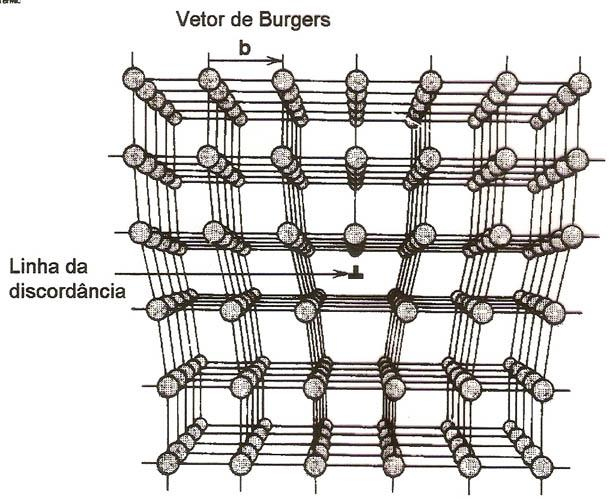
\includegraphics[scale=0.4,trim={0 0 0 0}]{figures/defLinhas}

\begin{itemize}
	\item Os defeitos (discordâncias, defeitos pontuais e contornos de grãos) atuam como barreiras para as discordâncias.
	\item O cisalhamento se dá mais facilmente nos planos de maior densidade atômica, que depende a orientação cristalográfica.
\end{itemize}


Fundamentos da Ciência e Eng. dos Materiais –uma abordagem integrada, Willian D. Callister, 2aed., Livros Técnicos e Científicos Editora, 2006.

Princípios de Ciência e Engenharia de Materiais. William F. Smith, 3ª ed, Editora Mc Graw Hill, 1998.

Ciência e Engenharia de Materiais: uma introdução, Willian D. Callister, 5a ed., Livros Técnicos e Científicos Editora, 2002.



{\large Direções Cristalinas Slide 04}

\section{Direções Cristalográficas}

\begin{itemize}
	\item Propriedades direcionais: Ex módulo de elasticidade do Fe maior na diagonal do cubo do que na aresta.
	\item Direções cristalinas são indexadas através de um segmento que se estende da origim até determinada posição dentro do cristal.
	\item Três índices são usados para designação das direções:

\end{itemize}


\begin{itemize}
	\item Índices de Müller$\rightarrow$ Base: célula unitária com sistema de coordenadas cartesianas, com origem em um vértice da célula.
	\begin{itemize}
		\item Vetor posicionado de forma a passar pela origem do sistema de coordenadas cartesianas. Pode ser transladado, desde que seja mantido um paralelismo com o vetor na origem.
		\item O comprimento da projeção do vetor em cada eixo é determinado em relação aos parâmetros de rede a, be c.
		\item Redução dos valores ao menor número inteiro por multiplicação ou divisão por um fator comum.
		\item Os três índices não são separados por vírgulas e ficam entre colchetes. [u v w]
		\item [u v w] correspondem às projeções nos eixos x, y e z, respectivamente.
	 	\item Em cristais cúbicos, as direções do tipo [111] (índices negativos e positivos) são iguais e identificadas por <111>.
	\end{itemize}	
\end{itemize}

{\large no slide 04 podemos achar alguns exemplos do índice de Müller para sólidos}


\section{Densidade de Sólidos}





\begin{itemize}
	\item \textbf{Densidade volumétrica}: $D_{v}$= massa por célula unitária / volume da célula unitária
	\item \textbf{Densidade Linear}: $D_{l}$= átomos centrados sobre o vetor direção / comprimento do vetor direção
\end{itemize}


{\large Slide 05. Planos Cristalinos e densidade planar}

\section{Planos cristalinos}
\noindent

Planos de átomos ou íons influenciam as propriedades e o comportamento dos materiais.

Os três índices não são separados por vírgulas e ficam entre parênteses.$\rightarrow$ (h k l)

Em cristais cúbicos, alguns planos constituem uma família de planos. \\ Ex: (100) (010) (001) etc $\rightarrow$ { h k l } Família de planos

No sistema hc os planos são designados por 4 índices (h k i l), que se referem a quatro eixos coordenados: 3 eixos na base do hexágono (120o entre si) e 1 eixo na vertical.


\section{Determinação do Índice de Müller - planos}


Os índices correspondem ao inverso das distâncias das interseções do plano com os eixos à origem.

São considerados os parâmetros de rede (a, b , c) como unidade para definição dos índices de Miller.

{\large CONSULTAR SLIDE PARA EXEMPLOS DE PLANOS CRISTALINOS}


\section{PLANOS CRISTALINOS vsCaracterização de estruturas}


\textbf{DIFRAÇÃO DE RAIOS-X} Técnica de caracterização estrutural de estruturas cristalinas. O bombardeamento de amostras com feixes de elétrons, gera emissão característica dos elementos constituintes.

A avaliação da estrutura cristalina pode ser feita por difratogramas produzidos por ondas que interagem com os átomos e que possuem comprimentos de onda com ordem de grandeza das distâncias interatômicas.

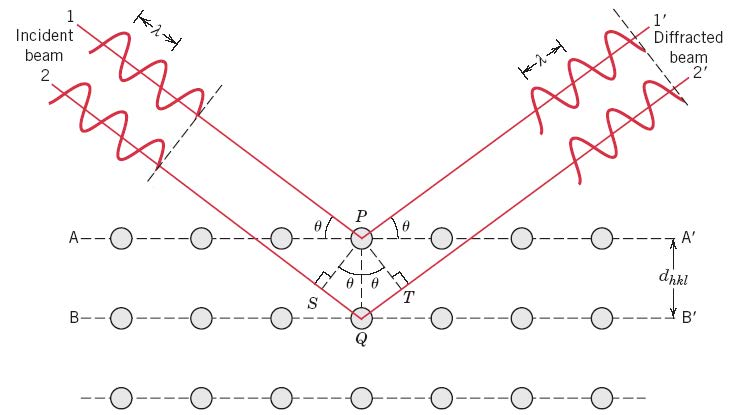
\includegraphics[scale=0.4,trim={0 0 0 0}]{figures/difracao}

Como funciona:

\begin{itemize}
	\item Incidência de feixe de raios-X com ângulo de incidência $\theta$sobre planos cristalinos com distância interplanar d.
	\item Emissão característica dos elementos constituintes.
\end{itemize}

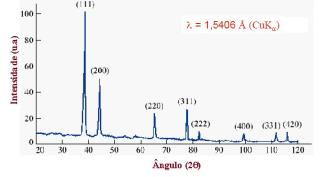
\includegraphics[scale=0.4,trim={0 0 0 0}]{figures/difratograma}

A avaliação da estrutura cristalina pode ser feita por difratogramas. Um feixe de raios-X é direcionado ao material cristalino e difratado pelos planos dos átomos ou íons com comprimentos de onda na ordem de grandeza das distâncias interatômicas.

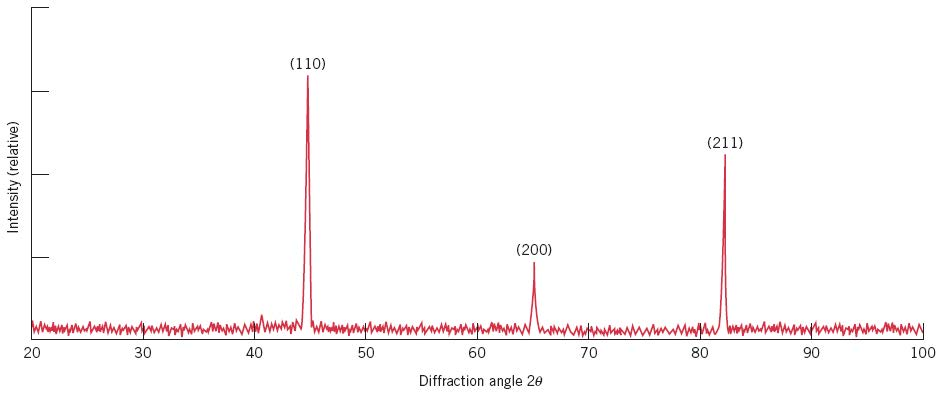
\includegraphics[scale=0.4,trim={0 0 0 0}]{figures/difraFe}

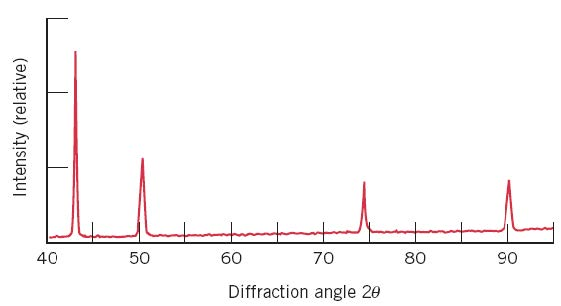
\includegraphics[scale=0.4,trim={0 0 0 0}]{figures/difraCu}

A mistura de amostras é revelada no difratograma com a superposição dos padrões individuais. Ex: Quartzo e NaCl (ver difratogramas do slide 05)


\textbf{Densidade planar}

$D_{p}$= átomos centrados sobre o plano / área do plano


{\large Slide 06. DIFUSÃO}


\section{Difusão em Sólidos}

\textit{Def:} O transporte de massa no sólido se dá através de movimento atômico.

Casos práticos:

\begin{itemize}
	\item Filtros para purificação de gases;
	\item Modificação superficial de peças;
	\item Dopagem de semicondutores;
	\item Revestimentos.
\end{itemize}



\subsection{Cementação}

\begin{itemize}
	\item Mdificação superficial de peças;
	\item Aumento do teor de C na parte mais externa de engrenagens para aumentar a dureza. Fonte de carbono: pó de grafite ou em fase liquida ou gasosa.
\end{itemize}


\subsection{Galvanização}

Imersão de pelas de aço em zinco fundido formando camadas de ligas Fe-Zn unidas metalurgicamente ao metal base. Temp. 445 a 455 $\degres$ C.

\subsection{Difusão L-L}
O potencia de difusão é dados pelo gradiente de concentração no sistema.


\subsection{Difusão S-S}

Objetivo: Equalização da composição química em ligas. PROCESSO TERMICAMENTE ATIVADO.

\subsubsection{Par de Difusão}

Duas barras de materiais metálicos  distintos sob o tratamento térmico. Concentrações de cobre e de níquel em função da posição no par de difusão. 

\textit{concentrações de cobre e de níquel em função da posição no par de difusão.}


\subsubsection{Condição para ocorrer difusão de átomos na rede cristalina}

\begin{itemize}
	\item Deve haver espaço livre (lacuna) adjacente ao átomo.
	\item O átomo que se desloca deve possuir energia suficiente para quebrar as ligações química que o une a seus átomos vizinhos .
	\item A movimentação dos átomos pode se dar pelo volume do material ou ao longo de defeitos cristalinos (mais rápida).
\end{itemize}


Mecanismos propostos:

\begin{enumerate}
	\item Difusão por lacunas (ou difusão substitucional)
	\item Difusão intersticial
	
\end{enumerate}


\begin{itemize}
	\item Difusão por lacunas (ou difusão substitucional): Átomo se desloca da posição padrão da rede cristalina para algum local (sitio) vazio próximo.
	\begin{itemize}
		\item O átomo segue direção contrária ao movimento da lacuna.
		\item Depende da quantidade de lacunas presentes na rede cristalina.
		\item A quantidade de lacunas aumenta com a temperatura.
		\item O processo é denominado AUTODIFUSÃO quando os próprios átomos da rede se difundem ou INTERDIFUSÃO quando ocorre difusão de impurezas substitucionais.
	\end{itemize}
	\item Difusão intersticial
	\begin{itemize}
		\item Átomos intersticiais migram para posições adjacentes da rede cristalina.
		\item Corresponde a um tipo importante de difusão em metais e ligas cuja impureza apresenta pequeno raio atômico em relação ao átomo da matriz cristalina. (ex: C e H)
		\item É geralmente mais rápida (apresenta maior coeficiente de difusão)
		\item Menor energia necessária para o movimento dos átomos.
	\end{itemize}
\end{itemize}

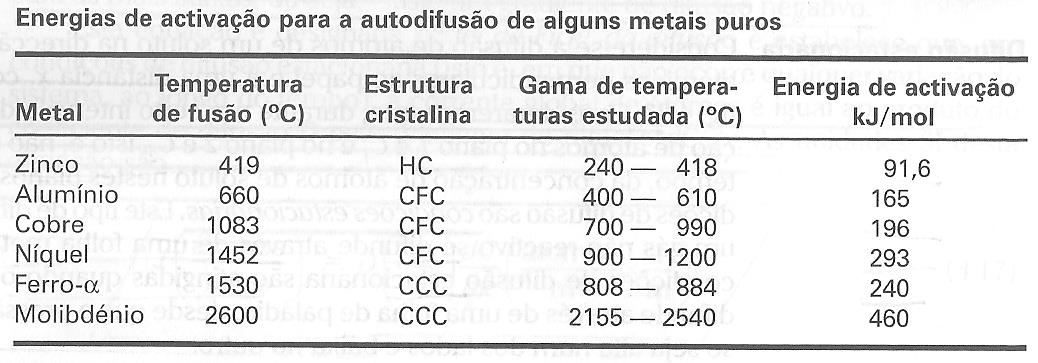
\includegraphics[scale=0.4,trim={0 0 0 0}]{figures/Eativacao}

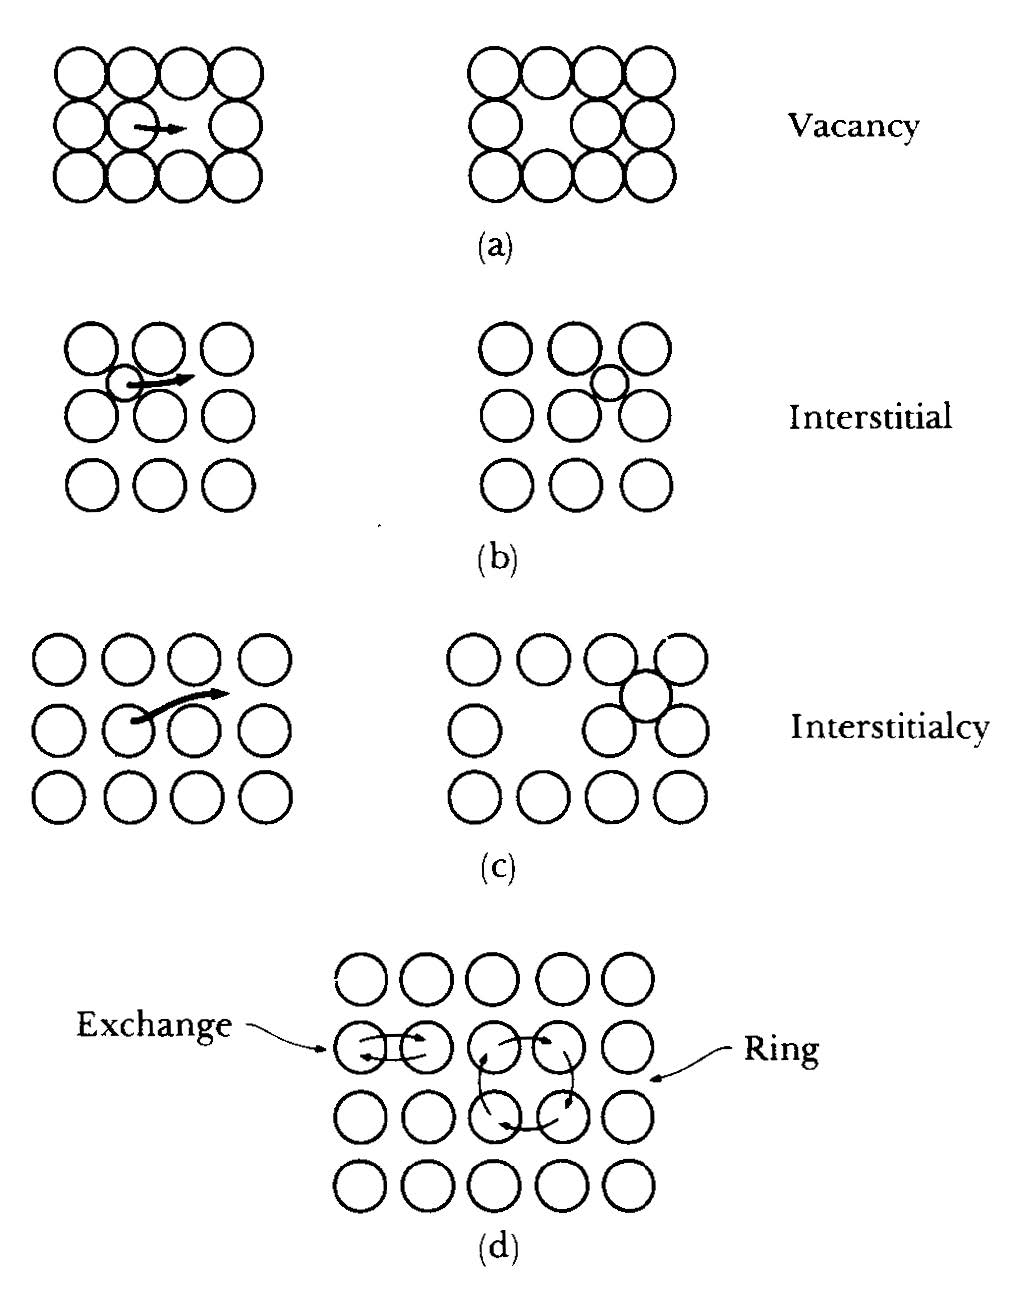
\includegraphics[scale=0.3,trim={0 0 0 0}]{figures/difusao}


\subsubsection{Fluxo de Difusão}

A velocidade com que ocorre a difusão é avaliada em termos de FLUXO DE DIFUSÃO que corresponde a massa (ou número de átomos) que se difunde por unidade de tempo através de uma área perpendicular à direção do movimento da massa que está se difundindo.

\begin{equation}\label{key}
J = \frac{M}{(A \cdot t)}
\end{equation}

onde: 

\begin{itemize}
	\item J = fluxo de difusão. $[\frac{Kg}{m^{2} \cdot s}]$ ou $[\frac{át}{m^{2} \cdot s}]$
	\item M = massa transportada (ou quantidade de átomos)
	\item A = área da seção transversal
	\item t = tempo
\end{itemize}



\subsubsection{title}


\subsubsection{title}



%\subsection*{Aussage}
%Eine Aussage ist ein Satz, der entweder wahr oder falsch ist, also nie beides zugleich.
%Wahre Aussagen haben den Wahrheitswert $w$ und falsche Aussagen den
%Wahrheitswert $f$.
%\subsection*{Belegung von Variablen}
%Sei $\mathcal{A}_B(F) = f$.
%Dann ist stets $\mathcal{A}_B(F\Rightarrow G) = w$
%\subsection*{Formelbeweis über Belegung}
%Wenn $F \wedge G$ eine Tautologie ist, dann (und nur dann) ist $F$ eine Tautologie und $G$ auch.
%Hinweis: In dem Lemma stecken zwei Teilaussagen, die beide zu beweisen sind:
%1. Wenn $F \wedge G$ eine Tautologie ist, dann ist $F$ eine Tautologie und $G$ auch.
%2. Umgekehrt: Sind $F$ und $G$ Tautologien, dann ist auch $F \wedge G$ eine.
%\emph{Beweis.}
%1. Annahme: $F \wedge G$ sei eine Tautologie.
%Dann: Für jede Belegung $B$ wertet $F \wedge G$ zu wahr aus.
%Dann: Das ist nur der Fall, wenn sowohl $F$ als auch $G$ (für jedes $B$) zu wahr auswerten.
%Dann: Für jede Belegung $B$ wertet $F$ zu wahr aus. Und:
%Für jede Belegung $B$ wertet $G$ zu wahr aus.
%Dann: $F$ ist Tautologie und $G$ ist Tautologie.
%2. Annahme: $F$ ist Tautologie und $G$ ist Tautologie.
%Dann: Für jede Belegung $B_1$ wertet $F$ zu wahr aus. Und: Für jede Belegung $B_2$ wertet $G$ zu wahr aus.
%Dann: Für jede Belegung $B$ wertet $F \wedge G$ zu wahr aus.
%Dann: $F \wedge G$ ist eine Tautologie.
%\subsection*{Äquivalenz und Folgerung}
%$p\equiv q$ gilt genau dann, wenn sowohl $p\models q$ als auch $q\models p$ gelten. \emph{Beweis.}
%$p\equiv q$ GDW $p\Leftrightarrow q$ ist Tautologie nach Def. von $\equiv$
%GDW $(p\Rightarrow q) \wedge (q\Rightarrow p)$ ist Tautologie
%GDW $(p\Rightarrow q)$ ist Tautologie und $(q\Rightarrow p)$ ist Tautologie
%GDW $(p\models q)$ gilt und $q\models p$ gilt.
%\subsection*{Substitution}
%Ersetzt man in einer Formel eine beliebige Teilformel $F$ durch eine logisch äquivalente
%Teilformel $F'$, so verändert sich der Wahrheitswerteverlauf der Gesamtformel nicht.
%Man kann Formeln also vereinfachen, indem man Teilformeln durch äquivalente
%(einfachere) Teilformeln ersetzt.
%\subsection*{Universum}
%Die freien Variablen in einer Aussagenform können durch Objekte aus einer als
%Universum bezeichneten Gesamtheit wie $\mathbb{N},\mathbb{R},\mathbb{Z},\mathbb{Q}$ ersetzt werden.
%\subsection*{Tautologien}
%$(p\wedge q)\Rightarrow p$\text{ bzw. }$p\Rightarrow (p\vee q)$\\
%$(q\Rightarrow p)\vee (\neg q\Rightarrow p)$\\
%$(p\Rightarrow q)\Leftrightarrow (\neg p\vee q)$\\
%$(p\Rightarrow q)\Leftrightarrow (\neg q\Rightarrow\neg p)$ \hfill\text{(Kontraposition)}\\
%$(p\wedge (p\Rightarrow q))\Rightarrow q$ \hfill\text{(Modus Ponens)}\\
%$((p\Rightarrow q)\wedge (q\Rightarrow r))\Rightarrow (p\Rightarrow r)$\\
%$((p\Rightarrow q)\wedge (p\Rightarrow r))\Rightarrow (p\Rightarrow (q\wedge r))$\\
%$((p\Rightarrow q)\wedge (q\Rightarrow p))\Leftrightarrow (p\Leftrightarrow q)$
%\subsection*{Nützliche Äquivalenzen}
%Kommutativität:\\
%$(p \wedge q) \equiv (q \wedge p)$\\
%$(p \vee q) \equiv (q \vee p)$\\
%Assoziativität:\\
%$(p \wedge (q \wedge r)) \equiv ((p \wedge q) \wedge r)$\\
%$(p \vee (q \vee r)) \equiv ((p \vee q) \vee r)$\\
%Distributivität:\\
%$(p \wedge (q \vee r)) \equiv ((p \wedge q) \vee (p \wedge r))$\\
%$(p \vee (q \wedge r)) \equiv ((p \vee q) \wedge (p \vee r))$\\
%Idempotenz:\\
%$(p \wedge p) \equiv p$\\
%$(p \vee p) \equiv p$\\
%Doppelnegation:\\
%$\neg (\neg p) \equiv p$\\
%de Morgans Regeln:\\
%$\neg (p \wedge q) \equiv ((\neg p) \vee (\neg q))$\\
%$\neg (p \vee q) \equiv ((\neg p) \wedge (\neg q))$\\
%Definition Implikation:\\
%$(p \Rightarrow q) \equiv (\neg p \vee q)$\\
%Tautologieregeln:\\
%$(p \wedge q) \equiv p$\hfill (falls $q$ eine Tautologie ist)\\
%$(p \vee q) \equiv q$\\
%Kontradiktionsregeln:\\
%$(p \wedge q) \equiv q$\hfill (falls $q$ eine Kontradiktion ist)\\
%$(p \vee q) \equiv p$\\
%Absorptionsregeln:\\
%$(p \wedge (p \vee q)) \equiv p$\\
%$(p \vee (p \wedge q)) \equiv p$\\
%Prinzip vom ausgeschlossenen Dritten:\\
%$p \vee (\neg p) \equiv w$\\\
%Prinzip vom ausgeschlossenen Widerspruch:\\
%$p \wedge (\neg p) \equiv f$
%\subsection*{Äquivalenzen von quant. Aussagen}
%Negationsregeln:\\
%$\neg\forall x:p(x)\equiv\exists x:(\neg p(x))$\\
%$\neg\exists x:p(x)\equiv\forall x:(\neg p(x))$\\
%Ausklammerregeln:\\
%$(\forall x:p(x)\wedge\forall y:q(y))\equiv\forall z:(p(z)\wedge q(z))$\\
%$(\exists x:p(x)\wedge\exists y:q(y))\equiv\exists z:(p(z)\wedge q(z))$\\
%Vertauschungsregeln\\
%$\forall x\forall y:p(x,y)\equiv\forall y\forall x:p(x,y)$\\
%$\exists x\exists y:p(x,y)\equiv\forall y\exists x:p(x,y)$
%\subsection*{Äquivalenzumformung}
%Wir demonstrieren an der Formel $\neg (\neg p \wedge q) \wedge (p \vee q)$, wie man mit Hilfe der
%aufgelisteten logischen Äquivalenzen tatsächlich zu Vereinfachungen kommen kann:\\
%$\phantom{{}\equiv{}} \neg (\neg p \wedge q) \wedge (p \vee q)$\\
%$\equiv (\neg (\neg p) \vee (\neg q)) \wedge (p \vee q)$\hfill de Morgan\\
%$\equiv (p \vee (\neg q)) \wedge (p \vee q)$\hfill Doppelnegation\\
%$\equiv p \vee ((\neg q) \wedge q)$\hfill Distributivtät v.r.n.l.\\
%$\equiv p \vee (q \wedge (\neg q))$\hfill Kommutativtät\\
%$\equiv p \vee f$\hfill Prinzip v. ausgeschl. Widerspruch\\
%$\equiv p$\hfill Kontradiktionsregel
%\subsection*{Quantifizierte Aussagen}
%Sei $p(x)$ eine Aussageform über dem Universum $U$.
%$\exists x : p(x)$ ist wahr genau dann, wenn ein $u$ in $U$ existiert, so dass $p(u)$ wahr ist.
%$\forall x : p(x)$ ist wahr genau dann, wenn $p(u)$ für jedes $u$ aus $U$ wahr ist.
